% Options for packages loaded elsewhere
\PassOptionsToPackage{unicode}{hyperref}
\PassOptionsToPackage{hyphens}{url}
\PassOptionsToPackage{dvipsnames,svgnames,x11names}{xcolor}
%
\documentclass[
  letterpaper,
  DIV=11,
  numbers=noendperiod]{scrreprt}

\usepackage{amsmath,amssymb}
\usepackage{lmodern}
\usepackage{iftex}
\ifPDFTeX
  \usepackage[T1]{fontenc}
  \usepackage[utf8]{inputenc}
  \usepackage{textcomp} % provide euro and other symbols
\else % if luatex or xetex
  \usepackage{unicode-math}
  \defaultfontfeatures{Scale=MatchLowercase}
  \defaultfontfeatures[\rmfamily]{Ligatures=TeX,Scale=1}
\fi
% Use upquote if available, for straight quotes in verbatim environments
\IfFileExists{upquote.sty}{\usepackage{upquote}}{}
\IfFileExists{microtype.sty}{% use microtype if available
  \usepackage[]{microtype}
  \UseMicrotypeSet[protrusion]{basicmath} % disable protrusion for tt fonts
}{}
\makeatletter
\@ifundefined{KOMAClassName}{% if non-KOMA class
  \IfFileExists{parskip.sty}{%
    \usepackage{parskip}
  }{% else
    \setlength{\parindent}{0pt}
    \setlength{\parskip}{6pt plus 2pt minus 1pt}}
}{% if KOMA class
  \KOMAoptions{parskip=half}}
\makeatother
\usepackage{xcolor}
\setlength{\emergencystretch}{3em} % prevent overfull lines
\setcounter{secnumdepth}{-\maxdimen} % remove section numbering
% Make \paragraph and \subparagraph free-standing
\ifx\paragraph\undefined\else
  \let\oldparagraph\paragraph
  \renewcommand{\paragraph}[1]{\oldparagraph{#1}\mbox{}}
\fi
\ifx\subparagraph\undefined\else
  \let\oldsubparagraph\subparagraph
  \renewcommand{\subparagraph}[1]{\oldsubparagraph{#1}\mbox{}}
\fi

\usepackage{color}
\usepackage{fancyvrb}
\newcommand{\VerbBar}{|}
\newcommand{\VERB}{\Verb[commandchars=\\\{\}]}
\DefineVerbatimEnvironment{Highlighting}{Verbatim}{commandchars=\\\{\}}
% Add ',fontsize=\small' for more characters per line
\usepackage{framed}
\definecolor{shadecolor}{RGB}{241,243,245}
\newenvironment{Shaded}{\begin{snugshade}}{\end{snugshade}}
\newcommand{\AlertTok}[1]{\textcolor[rgb]{0.68,0.00,0.00}{#1}}
\newcommand{\AnnotationTok}[1]{\textcolor[rgb]{0.37,0.37,0.37}{#1}}
\newcommand{\AttributeTok}[1]{\textcolor[rgb]{0.40,0.45,0.13}{#1}}
\newcommand{\BaseNTok}[1]{\textcolor[rgb]{0.68,0.00,0.00}{#1}}
\newcommand{\BuiltInTok}[1]{\textcolor[rgb]{0.00,0.23,0.31}{#1}}
\newcommand{\CharTok}[1]{\textcolor[rgb]{0.13,0.47,0.30}{#1}}
\newcommand{\CommentTok}[1]{\textcolor[rgb]{0.37,0.37,0.37}{#1}}
\newcommand{\CommentVarTok}[1]{\textcolor[rgb]{0.37,0.37,0.37}{\textit{#1}}}
\newcommand{\ConstantTok}[1]{\textcolor[rgb]{0.56,0.35,0.01}{#1}}
\newcommand{\ControlFlowTok}[1]{\textcolor[rgb]{0.00,0.23,0.31}{#1}}
\newcommand{\DataTypeTok}[1]{\textcolor[rgb]{0.68,0.00,0.00}{#1}}
\newcommand{\DecValTok}[1]{\textcolor[rgb]{0.68,0.00,0.00}{#1}}
\newcommand{\DocumentationTok}[1]{\textcolor[rgb]{0.37,0.37,0.37}{\textit{#1}}}
\newcommand{\ErrorTok}[1]{\textcolor[rgb]{0.68,0.00,0.00}{#1}}
\newcommand{\ExtensionTok}[1]{\textcolor[rgb]{0.00,0.23,0.31}{#1}}
\newcommand{\FloatTok}[1]{\textcolor[rgb]{0.68,0.00,0.00}{#1}}
\newcommand{\FunctionTok}[1]{\textcolor[rgb]{0.28,0.35,0.67}{#1}}
\newcommand{\ImportTok}[1]{\textcolor[rgb]{0.00,0.46,0.62}{#1}}
\newcommand{\InformationTok}[1]{\textcolor[rgb]{0.37,0.37,0.37}{#1}}
\newcommand{\KeywordTok}[1]{\textcolor[rgb]{0.00,0.23,0.31}{#1}}
\newcommand{\NormalTok}[1]{\textcolor[rgb]{0.00,0.23,0.31}{#1}}
\newcommand{\OperatorTok}[1]{\textcolor[rgb]{0.37,0.37,0.37}{#1}}
\newcommand{\OtherTok}[1]{\textcolor[rgb]{0.00,0.23,0.31}{#1}}
\newcommand{\PreprocessorTok}[1]{\textcolor[rgb]{0.68,0.00,0.00}{#1}}
\newcommand{\RegionMarkerTok}[1]{\textcolor[rgb]{0.00,0.23,0.31}{#1}}
\newcommand{\SpecialCharTok}[1]{\textcolor[rgb]{0.37,0.37,0.37}{#1}}
\newcommand{\SpecialStringTok}[1]{\textcolor[rgb]{0.13,0.47,0.30}{#1}}
\newcommand{\StringTok}[1]{\textcolor[rgb]{0.13,0.47,0.30}{#1}}
\newcommand{\VariableTok}[1]{\textcolor[rgb]{0.07,0.07,0.07}{#1}}
\newcommand{\VerbatimStringTok}[1]{\textcolor[rgb]{0.13,0.47,0.30}{#1}}
\newcommand{\WarningTok}[1]{\textcolor[rgb]{0.37,0.37,0.37}{\textit{#1}}}

\providecommand{\tightlist}{%
  \setlength{\itemsep}{0pt}\setlength{\parskip}{0pt}}\usepackage{longtable,booktabs,array}
\usepackage{calc} % for calculating minipage widths
% Correct order of tables after \paragraph or \subparagraph
\usepackage{etoolbox}
\makeatletter
\patchcmd\longtable{\par}{\if@noskipsec\mbox{}\fi\par}{}{}
\makeatother
% Allow footnotes in longtable head/foot
\IfFileExists{footnotehyper.sty}{\usepackage{footnotehyper}}{\usepackage{footnote}}
\makesavenoteenv{longtable}
\usepackage{graphicx}
\makeatletter
\def\maxwidth{\ifdim\Gin@nat@width>\linewidth\linewidth\else\Gin@nat@width\fi}
\def\maxheight{\ifdim\Gin@nat@height>\textheight\textheight\else\Gin@nat@height\fi}
\makeatother
% Scale images if necessary, so that they will not overflow the page
% margins by default, and it is still possible to overwrite the defaults
% using explicit options in \includegraphics[width, height, ...]{}
\setkeys{Gin}{width=\maxwidth,height=\maxheight,keepaspectratio}
% Set default figure placement to htbp
\makeatletter
\def\fps@figure{htbp}
\makeatother

\KOMAoption{captions}{tableheading}
\makeatletter
\@ifpackageloaded{tcolorbox}{}{\usepackage[many]{tcolorbox}}
\@ifpackageloaded{fontawesome5}{}{\usepackage{fontawesome5}}
\definecolor{quarto-callout-color}{HTML}{909090}
\definecolor{quarto-callout-note-color}{HTML}{0758E5}
\definecolor{quarto-callout-important-color}{HTML}{CC1914}
\definecolor{quarto-callout-warning-color}{HTML}{EB9113}
\definecolor{quarto-callout-tip-color}{HTML}{00A047}
\definecolor{quarto-callout-caution-color}{HTML}{FC5300}
\definecolor{quarto-callout-color-frame}{HTML}{acacac}
\definecolor{quarto-callout-note-color-frame}{HTML}{4582ec}
\definecolor{quarto-callout-important-color-frame}{HTML}{d9534f}
\definecolor{quarto-callout-warning-color-frame}{HTML}{f0ad4e}
\definecolor{quarto-callout-tip-color-frame}{HTML}{02b875}
\definecolor{quarto-callout-caution-color-frame}{HTML}{fd7e14}
\makeatother
\makeatletter
\makeatother
\makeatletter
\makeatother
\makeatletter
\@ifpackageloaded{caption}{}{\usepackage{caption}}
\AtBeginDocument{%
\ifdefined\contentsname
  \renewcommand*\contentsname{Table of contents}
\else
  \newcommand\contentsname{Table of contents}
\fi
\ifdefined\listfigurename
  \renewcommand*\listfigurename{List of Figures}
\else
  \newcommand\listfigurename{List of Figures}
\fi
\ifdefined\listtablename
  \renewcommand*\listtablename{List of Tables}
\else
  \newcommand\listtablename{List of Tables}
\fi
\ifdefined\figurename
  \renewcommand*\figurename{Figure}
\else
  \newcommand\figurename{Figure}
\fi
\ifdefined\tablename
  \renewcommand*\tablename{Table}
\else
  \newcommand\tablename{Table}
\fi
}
\@ifpackageloaded{float}{}{\usepackage{float}}
\floatstyle{ruled}
\@ifundefined{c@chapter}{\newfloat{codelisting}{h}{lop}}{\newfloat{codelisting}{h}{lop}[chapter]}
\floatname{codelisting}{Listing}
\newcommand*\listoflistings{\listof{codelisting}{List of Listings}}
\makeatother
\makeatletter
\@ifpackageloaded{caption}{}{\usepackage{caption}}
\@ifpackageloaded{subcaption}{}{\usepackage{subcaption}}
\makeatother
\makeatletter
\@ifpackageloaded{tcolorbox}{}{\usepackage[many]{tcolorbox}}
\makeatother
\makeatletter
\@ifundefined{shadecolor}{\definecolor{shadecolor}{rgb}{.97, .97, .97}}
\makeatother
\makeatletter
\makeatother
\ifLuaTeX
  \usepackage{selnolig}  % disable illegal ligatures
\fi
\IfFileExists{bookmark.sty}{\usepackage{bookmark}}{\usepackage{hyperref}}
\IfFileExists{xurl.sty}{\usepackage{xurl}}{} % add URL line breaks if available
\urlstyle{same} % disable monospaced font for URLs
\hypersetup{
  colorlinks=true,
  linkcolor={blue},
  filecolor={Maroon},
  citecolor={Blue},
  urlcolor={Blue},
  pdfcreator={LaTeX via pandoc}}

\author{}
\date{}

\begin{document}
\ifdefined\Shaded\renewenvironment{Shaded}{\begin{tcolorbox}[borderline west={3pt}{0pt}{shadecolor}, enhanced, breakable, boxrule=0pt, frame hidden, interior hidden, sharp corners]}{\end{tcolorbox}}\fi

\hypertarget{sec-join}{%
\chapter{Joining data}\label{sec-join}}

\hypertarget{merging-two-related-tables-into-one}{%
\section{Merging two related tables into
one}\label{merging-two-related-tables-into-one}}

So far, we have been working with a single table of data at a time.
Often however, information about the same thing is scattered across
multiple tables and files. In such cases, we sometimes want to
\emph{join} those separate tables into a single one. To illustrate how
this can be done, let us create two simple tables. The first will
contain the names of students, along with their chosen subject:

\begin{Shaded}
\begin{Highlighting}[]
\FunctionTok{library}\NormalTok{(tidyverse)}

\NormalTok{studies }\OtherTok{\textless{}{-}} \FunctionTok{tibble}\NormalTok{(}\AttributeTok{name    =} \FunctionTok{c}\NormalTok{(}\StringTok{"Sacha"}\NormalTok{, }\StringTok{"Gabe"}\NormalTok{, }\StringTok{"Alex"}\NormalTok{),}
                  \AttributeTok{subject =} \FunctionTok{c}\NormalTok{(}\StringTok{"Physics"}\NormalTok{, }\StringTok{"Chemistry"}\NormalTok{, }\StringTok{"Biology"}\NormalTok{))}
\FunctionTok{print}\NormalTok{(studies)}
\end{Highlighting}
\end{Shaded}

\begin{verbatim}
# A tibble: 3 x 2
  name  subject  
  <chr> <chr>    
1 Sacha Physics  
2 Gabe  Chemistry
3 Alex  Biology  
\end{verbatim}

The second table contains slightly different information: it holds which
year a given student is currently into their studies.

\begin{Shaded}
\begin{Highlighting}[]
\NormalTok{stage }\OtherTok{\textless{}{-}} \FunctionTok{tibble}\NormalTok{(}\AttributeTok{name =} \FunctionTok{c}\NormalTok{(}\StringTok{"Sacha"}\NormalTok{, }\StringTok{"Alex"}\NormalTok{, }\StringTok{"Jamie"}\NormalTok{),}
                \AttributeTok{year =} \FunctionTok{c}\NormalTok{(}\DecValTok{3}\NormalTok{, }\DecValTok{1}\NormalTok{, }\DecValTok{2}\NormalTok{))}
\FunctionTok{print}\NormalTok{(stage)}
\end{Highlighting}
\end{Shaded}

\begin{verbatim}
# A tibble: 3 x 2
  name   year
  <chr> <dbl>
1 Sacha     3
2 Alex      1
3 Jamie     2
\end{verbatim}

Notice that, while Sacha and Alex appear in both tables, Gabe is only
included in \texttt{studies} and Jamie only in \texttt{stage}. While in
such tiny datasets this might seem like an avoidable oversight, such
non-perfect alignment of data can be the norm when working with data
spanning hundreds, thousands, or more rows. Here, for the purposes of
illustration, we use small tables, but the principles we learn here
apply in a broader context as well.

There are four commonly used ways of joining these tables into one
single dataset. All of them follow the same general pattern: the
arguments are two tibbles (or data frames) to be joined, plus a
\texttt{by\ =} argument which lists the name(s) of the column(s) based
on which the tables should be joined. The output is always a single
tibble (data frame), containing some type of joining of the data. Let us
now look at each joining method in detail.

\hypertarget{left_join}{%
\subsection{\texorpdfstring{\texttt{left\_join}}{left\_join}}\label{left_join}}

The \texttt{left\_join} function keeps only those rows that appear in
the \emph{first} of the two tables to be joined:

\begin{Shaded}
\begin{Highlighting}[]
\FunctionTok{left\_join}\NormalTok{(studies, stage, }\AttributeTok{by =} \StringTok{"name"}\NormalTok{)}
\end{Highlighting}
\end{Shaded}

\begin{verbatim}
# A tibble: 3 x 3
  name  subject    year
  <chr> <chr>     <dbl>
1 Sacha Physics       3
2 Gabe  Chemistry    NA
3 Alex  Biology       1
\end{verbatim}

There are two things to notice. First, Jamie is missing from the
\texttt{name} column above, even though s/he did appear in the
\texttt{stage} tibble. This is exactly the point of \texttt{left\_join}:
if a row entry in the joining column (specified in \texttt{by\ =}) does
not appear in the \emph{first} table listed in the arguments (here, the
\texttt{name} column of \texttt{studies}), then it is omitted. Second,
the \texttt{year} entry for Gabe is \texttt{NA}. This is because Gabe is
absent from the \texttt{stage} table, and therefore has no associated
year of study. Rather than make up nonsense, R fills out such missing
data with \texttt{NA} values.

\hypertarget{right_join}{%
\subsection{\texorpdfstring{\texttt{right\_join}}{right\_join}}\label{right_join}}

This function works just like \texttt{left\_join}, except only those
rows are retained which appear in the \emph{second} of the two tables to
be joined:

\begin{Shaded}
\begin{Highlighting}[]
\FunctionTok{right\_join}\NormalTok{(studies, stage, }\AttributeTok{by =} \StringTok{"name"}\NormalTok{)}
\end{Highlighting}
\end{Shaded}

\begin{verbatim}
# A tibble: 3 x 3
  name  subject  year
  <chr> <chr>   <dbl>
1 Sacha Physics     3
2 Alex  Biology     1
3 Jamie <NA>        2
\end{verbatim}

In other words, this is exactly the same as calling \texttt{left\_join}
with its first two arguments reversed:

\begin{Shaded}
\begin{Highlighting}[]
\FunctionTok{left\_join}\NormalTok{(stage, studies, }\AttributeTok{by =} \StringTok{"name"}\NormalTok{)}
\end{Highlighting}
\end{Shaded}

\begin{verbatim}
# A tibble: 3 x 3
  name   year subject
  <chr> <dbl> <chr>  
1 Sacha     3 Physics
2 Alex      1 Biology
3 Jamie     2 <NA>   
\end{verbatim}

The only difference is in the ordering of the columns, but the data
contained in the tables are identical.

In this case, the columns \texttt{subject} is \texttt{NA} for Jamie. The
reason is the same as it was before: since the \texttt{studies} table
has no \texttt{name} entry for Jamie, the corresponding subject area is
filled in with a missing value \texttt{NA}.

\hypertarget{inner_join}{%
\subsection{\texorpdfstring{\texttt{inner\_join}}{inner\_join}}\label{inner_join}}

This function retains only those rows which appear in \emph{both} tables
to be joined. For our example, since Gabe only appears in
\texttt{studies} and Jamie only in \texttt{stage}, they will be dropped
by \texttt{inner\_join} and only Sacha and Alex are retained (since they
appear in both tables):

\begin{Shaded}
\begin{Highlighting}[]
\FunctionTok{inner\_join}\NormalTok{(studies, stage, }\AttributeTok{by =} \StringTok{"name"}\NormalTok{)}
\end{Highlighting}
\end{Shaded}

\begin{verbatim}
# A tibble: 2 x 3
  name  subject  year
  <chr> <chr>   <dbl>
1 Sacha Physics     3
2 Alex  Biology     1
\end{verbatim}

\hypertarget{full_join}{%
\subsection{\texorpdfstring{\texttt{full\_join}}{full\_join}}\label{full_join}}

The complement to \texttt{inner\_join}, this function retains all rows
in all tables, filling in missing values with \texttt{NA}s everywhere:

\begin{Shaded}
\begin{Highlighting}[]
\FunctionTok{full\_join}\NormalTok{(studies, stage, }\AttributeTok{by =} \StringTok{"name"}\NormalTok{)}
\end{Highlighting}
\end{Shaded}

\begin{verbatim}
# A tibble: 4 x 3
  name  subject    year
  <chr> <chr>     <dbl>
1 Sacha Physics       3
2 Gabe  Chemistry    NA
3 Alex  Biology       1
4 Jamie <NA>          2
\end{verbatim}

A useful table summarizing these options, taken from a more
comprehensive (though slightly out-of-date)
\href{https://www.rstudio.com/wp-content/uploads/2015/02/data-wrangling-cheatsheet.pdf}{cheat
sheet}, is below:

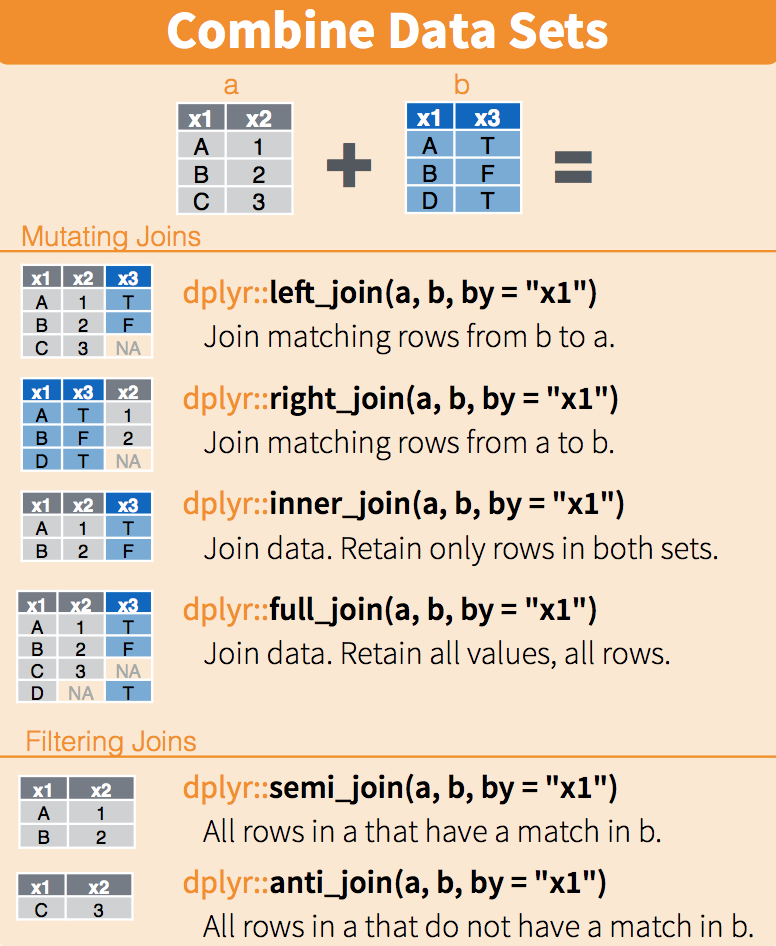
\includegraphics[width=0.7\textwidth,height=\textheight]{joins.png}

(As you see, apart from the four so-called \emph{mutating joins} we have
learned about, there are also two \emph{filtering joins} included in
this cheat sheet as well. We will not be covering those here, but feel
free to check out their help pages.)

\hypertarget{joining-by-multiple-columns}{%
\subsection{Joining by multiple
columns}\label{joining-by-multiple-columns}}

It is also possible to use the above joining functions specifying
multiple columns to join data by. To illustrate how to do this and what
this means, imagine that we slightly modify the student data. The first
table will contain the name, study area, and year of study for each
student. The second table will contain the name and study area of each
student, plus whether they have passed their most recent exam:

\begin{Shaded}
\begin{Highlighting}[]
\NormalTok{program  }\OtherTok{\textless{}{-}} \FunctionTok{tibble}\NormalTok{(}\AttributeTok{name     =} \FunctionTok{c}\NormalTok{(}\StringTok{"Sacha"}\NormalTok{, }\StringTok{"Gabe"}\NormalTok{, }\StringTok{"Alex"}\NormalTok{),}
                   \AttributeTok{subject  =} \FunctionTok{c}\NormalTok{(}\StringTok{"Physics"}\NormalTok{, }\StringTok{"Chemistry"}\NormalTok{, }\StringTok{"Biology"}\NormalTok{),}
                   \AttributeTok{year     =} \FunctionTok{c}\NormalTok{(}\DecValTok{1}\NormalTok{, }\DecValTok{3}\NormalTok{, }\DecValTok{2}\NormalTok{))}
\FunctionTok{print}\NormalTok{(program)}
\end{Highlighting}
\end{Shaded}

\begin{verbatim}
# A tibble: 3 x 3
  name  subject    year
  <chr> <chr>     <dbl>
1 Sacha Physics       1
2 Gabe  Chemistry     3
3 Alex  Biology       2
\end{verbatim}

\begin{Shaded}
\begin{Highlighting}[]
\NormalTok{progress }\OtherTok{\textless{}{-}} \FunctionTok{tibble}\NormalTok{(}\AttributeTok{name     =} \FunctionTok{c}\NormalTok{(}\StringTok{"Sacha"}\NormalTok{, }\StringTok{"Gabe"}\NormalTok{, }\StringTok{"Jamie"}\NormalTok{),}
                   \AttributeTok{subject  =} \FunctionTok{c}\NormalTok{(}\StringTok{"Physics"}\NormalTok{, }\StringTok{"Chemistry"}\NormalTok{, }\StringTok{"Biology"}\NormalTok{),}
                   \AttributeTok{examPass =} \FunctionTok{c}\NormalTok{(}\ConstantTok{TRUE}\NormalTok{, }\ConstantTok{FALSE}\NormalTok{, }\ConstantTok{TRUE}\NormalTok{))}
\FunctionTok{print}\NormalTok{(progress)}
\end{Highlighting}
\end{Shaded}

\begin{verbatim}
# A tibble: 3 x 3
  name  subject   examPass
  <chr> <chr>     <lgl>   
1 Sacha Physics   TRUE    
2 Gabe  Chemistry FALSE   
3 Jamie Biology   TRUE    
\end{verbatim}

And now, since the tables share not just one but two columns, it makes
sense to join them using both. This can be done by specifying each
column inside a vector in the \texttt{by\ =} argument. For example,
left-joining \texttt{program} and \texttt{progress} by both
\texttt{name} and \texttt{subject} leads to a joint table in which all
unique \texttt{name}-\texttt{subject} combinations found in
\texttt{program} are retained, but those found only in \texttt{progress}
are discarded:

\begin{Shaded}
\begin{Highlighting}[]
\FunctionTok{left\_join}\NormalTok{(program, progress, }\AttributeTok{by =} \FunctionTok{c}\NormalTok{(}\StringTok{"name"}\NormalTok{, }\StringTok{"subject"}\NormalTok{))}
\end{Highlighting}
\end{Shaded}

\begin{verbatim}
# A tibble: 3 x 4
  name  subject    year examPass
  <chr> <chr>     <dbl> <lgl>   
1 Sacha Physics       1 TRUE    
2 Gabe  Chemistry     3 FALSE   
3 Alex  Biology       2 NA      
\end{verbatim}

\begin{tcolorbox}[enhanced jigsaw, leftrule=.75mm, rightrule=.15mm, breakable, titlerule=0mm, colframe=quarto-callout-warning-color-frame, left=2mm, opacityback=0, coltitle=black, colback=white, title=\textcolor{quarto-callout-warning-color}{\faExclamationTriangle}\hspace{0.5em}{Warning}, bottomtitle=1mm, colbacktitle=quarto-callout-warning-color!10!white, arc=.35mm, toptitle=1mm, bottomrule=.15mm, toprule=.15mm, opacitybacktitle=0.6]
As mentioned, the columns by which one joins the tables must be included
in a vector. Forgetting to do this will either fail or produce faulty
output:

\begin{Shaded}
\begin{Highlighting}[]
\FunctionTok{left\_join}\NormalTok{(program, progress, }\AttributeTok{by =} \StringTok{"name"}\NormalTok{, }\StringTok{"subject"}\NormalTok{)}
\end{Highlighting}
\end{Shaded}

\begin{verbatim}
# A tibble: 3 x 5
  name  subject.x  year subject.y examPass
  <chr> <chr>     <dbl> <chr>     <lgl>   
1 Sacha Physics       1 Physics   TRUE    
2 Gabe  Chemistry     3 Chemistry FALSE   
3 Alex  Biology       2 <NA>      NA      
\end{verbatim}

The problem is that the comma after \texttt{name} is interpreted as the
start of the next argument to \texttt{left\_join}, instead of being a
part of the \texttt{by\ =} argument. Again, the solution is simple:
enclose multiple column names in a vector.
\end{tcolorbox}

The other joining functions also work as expected:

\begin{Shaded}
\begin{Highlighting}[]
\FunctionTok{right\_join}\NormalTok{(program, progress, }\AttributeTok{by =} \FunctionTok{c}\NormalTok{(}\StringTok{"name"}\NormalTok{, }\StringTok{"subject"}\NormalTok{))}
\end{Highlighting}
\end{Shaded}

\begin{verbatim}
# A tibble: 3 x 4
  name  subject    year examPass
  <chr> <chr>     <dbl> <lgl>   
1 Sacha Physics       1 TRUE    
2 Gabe  Chemistry     3 FALSE   
3 Jamie Biology      NA TRUE    
\end{verbatim}

\begin{Shaded}
\begin{Highlighting}[]
\FunctionTok{inner\_join}\NormalTok{(program, progress, }\AttributeTok{by =} \FunctionTok{c}\NormalTok{(}\StringTok{"name"}\NormalTok{, }\StringTok{"subject"}\NormalTok{))}
\end{Highlighting}
\end{Shaded}

\begin{verbatim}
# A tibble: 2 x 4
  name  subject    year examPass
  <chr> <chr>     <dbl> <lgl>   
1 Sacha Physics       1 TRUE    
2 Gabe  Chemistry     3 FALSE   
\end{verbatim}

\begin{Shaded}
\begin{Highlighting}[]
\FunctionTok{full\_join}\NormalTok{(program, progress, }\AttributeTok{by =} \FunctionTok{c}\NormalTok{(}\StringTok{"name"}\NormalTok{, }\StringTok{"subject"}\NormalTok{))}
\end{Highlighting}
\end{Shaded}

\begin{verbatim}
# A tibble: 4 x 4
  name  subject    year examPass
  <chr> <chr>     <dbl> <lgl>   
1 Sacha Physics       1 TRUE    
2 Gabe  Chemistry     3 FALSE   
3 Alex  Biology       2 NA      
4 Jamie Biology      NA TRUE    
\end{verbatim}

\hypertarget{binding-rows-and-columns-to-a-table}{%
\section{Binding rows and columns to a
table}\label{binding-rows-and-columns-to-a-table}}

Occasionally, a simpler problem presents itself: there is a single
dataset, but its rows are contained across separate tables. For example,
a table containing student names and subject areas might be spread
across two tables, like this:

\begin{Shaded}
\begin{Highlighting}[]
\NormalTok{studies1 }\OtherTok{\textless{}{-}} \FunctionTok{tibble}\NormalTok{(}\AttributeTok{name    =} \FunctionTok{c}\NormalTok{(}\StringTok{"Sacha"}\NormalTok{, }\StringTok{"Gabe"}\NormalTok{, }\StringTok{"Alex"}\NormalTok{),}
                   \AttributeTok{subject =} \FunctionTok{c}\NormalTok{(}\StringTok{"Physics"}\NormalTok{, }\StringTok{"Chemistry"}\NormalTok{, }\StringTok{"Biology"}\NormalTok{))}
\FunctionTok{print}\NormalTok{(studies1)}
\end{Highlighting}
\end{Shaded}

\begin{verbatim}
# A tibble: 3 x 2
  name  subject  
  <chr> <chr>    
1 Sacha Physics  
2 Gabe  Chemistry
3 Alex  Biology  
\end{verbatim}

\begin{Shaded}
\begin{Highlighting}[]
\NormalTok{studies2 }\OtherTok{\textless{}{-}} \FunctionTok{tibble}\NormalTok{(}\AttributeTok{name    =} \FunctionTok{c}\NormalTok{(}\StringTok{"Jamie"}\NormalTok{, }\StringTok{"Ashley"}\NormalTok{, }\StringTok{"Dallas"}\NormalTok{, }\StringTok{"Jordan"}\NormalTok{),}
                   \AttributeTok{subject =} \FunctionTok{c}\NormalTok{(}\StringTok{"Geology"}\NormalTok{, }\StringTok{"Mathematics"}\NormalTok{, }\StringTok{"Philosophy"}\NormalTok{, }\StringTok{"Physics"}\NormalTok{))}
\FunctionTok{print}\NormalTok{(studies2)}
\end{Highlighting}
\end{Shaded}

\begin{verbatim}
# A tibble: 4 x 2
  name   subject    
  <chr>  <chr>      
1 Jamie  Geology    
2 Ashley Mathematics
3 Dallas Philosophy 
4 Jordan Physics    
\end{verbatim}

The tables have the exact same structure, in that the column names and
types are identical. It's just that the rows are, for some reason,
disparate. To combine them together, we could recourse to full-joining
the tables by both their columns:

\begin{Shaded}
\begin{Highlighting}[]
\FunctionTok{full\_join}\NormalTok{(studies1, studies2, }\AttributeTok{by =} \FunctionTok{c}\NormalTok{(}\StringTok{"name"}\NormalTok{, }\StringTok{"subject"}\NormalTok{))}
\end{Highlighting}
\end{Shaded}

\begin{verbatim}
# A tibble: 7 x 2
  name   subject    
  <chr>  <chr>      
1 Sacha  Physics    
2 Gabe   Chemistry  
3 Alex   Biology    
4 Jamie  Geology    
5 Ashley Mathematics
6 Dallas Philosophy 
7 Jordan Physics    
\end{verbatim}

This, however, is not necessary. Whenever all we need to do is take two
tables and stick their rows together, there is the simpler
\texttt{bind\_rows}:

\begin{Shaded}
\begin{Highlighting}[]
\FunctionTok{bind\_rows}\NormalTok{(studies1, studies2)}
\end{Highlighting}
\end{Shaded}

\begin{verbatim}
# A tibble: 7 x 2
  name   subject    
  <chr>  <chr>      
1 Sacha  Physics    
2 Gabe   Chemistry  
3 Alex   Biology    
4 Jamie  Geology    
5 Ashley Mathematics
6 Dallas Philosophy 
7 Jordan Physics    
\end{verbatim}

Similarly, in case two tables have the same number of rows but different
columns, one can stick their columns together using \texttt{bind\_cols}.
For example, suppose we have

\begin{Shaded}
\begin{Highlighting}[]
\NormalTok{studies }\OtherTok{\textless{}{-}} \FunctionTok{tibble}\NormalTok{(}\AttributeTok{name    =} \FunctionTok{c}\NormalTok{(}\StringTok{"Sacha"}\NormalTok{, }\StringTok{"Gabe"}\NormalTok{, }\StringTok{"Alex"}\NormalTok{),}
                  \AttributeTok{subject =} \FunctionTok{c}\NormalTok{(}\StringTok{"Physics"}\NormalTok{, }\StringTok{"Chemistry"}\NormalTok{, }\StringTok{"Biology"}\NormalTok{))}
\FunctionTok{print}\NormalTok{(studies)}
\end{Highlighting}
\end{Shaded}

\begin{verbatim}
# A tibble: 3 x 2
  name  subject  
  <chr> <chr>    
1 Sacha Physics  
2 Gabe  Chemistry
3 Alex  Biology  
\end{verbatim}

as well as a table with year of study and result of last exam only:

\begin{Shaded}
\begin{Highlighting}[]
\NormalTok{yearExam }\OtherTok{\textless{}{-}} \FunctionTok{tibble}\NormalTok{(}\AttributeTok{year     =} \FunctionTok{c}\NormalTok{(}\DecValTok{3}\NormalTok{, }\DecValTok{1}\NormalTok{, }\DecValTok{2}\NormalTok{),}
                   \AttributeTok{examPass =} \FunctionTok{c}\NormalTok{(}\ConstantTok{FALSE}\NormalTok{, }\ConstantTok{TRUE}\NormalTok{, }\ConstantTok{TRUE}\NormalTok{))}
\FunctionTok{print}\NormalTok{(yearExam)}
\end{Highlighting}
\end{Shaded}

\begin{verbatim}
# A tibble: 3 x 2
   year examPass
  <dbl> <lgl>   
1     3 FALSE   
2     1 TRUE    
3     2 TRUE    
\end{verbatim}

We can now join these using \texttt{bind\_cols}:

\begin{Shaded}
\begin{Highlighting}[]
\FunctionTok{bind\_cols}\NormalTok{(studies, yearExam)}
\end{Highlighting}
\end{Shaded}

\begin{verbatim}
# A tibble: 3 x 4
  name  subject    year examPass
  <chr> <chr>     <dbl> <lgl>   
1 Sacha Physics       3 FALSE   
2 Gabe  Chemistry     1 TRUE    
3 Alex  Biology       2 TRUE    
\end{verbatim}

\hypertarget{exercises}{%
\section{Exercises}\label{exercises}}

We have used the data of Fauchald et al.~(2017)\footnote{Fauchald, P. et
  al.~(2017). Arctic greening from warming promotes declines in caribou
  populations. \emph{Science Advances}, 3:e1601365.} before in other
exercises. As a reminder, they tracked the population size of various
herds of caribou in North America over time, and correlated population
cycling with the amount of vegetation and sea-ice cover. Two files from
their data are on Lisam: \texttt{pop\_size.tsv} (herd population sizes),
and \texttt{sea\_ice.tsv} (sea ice cover per year and month).

\begin{enumerate}
\def\labelenumi{\arabic{enumi}.}
\tightlist
\item
  Load these two datasets into two variables. They could be called
  \texttt{pop} and \texttt{ice}, for instance. Look at the data to
  familiarize yourself with them. How many rows and columns are in each?
\item
  Before doing anything else: how many rows will there be in the table
  that is the left join of \texttt{pop} and \texttt{ice}, based on the
  two columns \texttt{Herd} and \texttt{Year}? Perform the left join to
  see if you were correct. Where do you see \texttt{NA}s in the table,
  and why?
\item
  Now do the same with right-joining, inner-joining, and full-joining
  \texttt{pop} and \texttt{ice}.
\end{enumerate}



\end{document}
